% ── Section 3: Methodology ──────────────────────────────────────────────────
\section{Methodology}
\label{sec:methodology}

\subsection{Overview and Pipeline Flow}
The multimodal digital twin framework is structured as a hierarchical, multi-stage prognostic pipeline that mirrors clinical decision-making under real-world observational constraints (Fig.~\ref{fig:architecture}). Rather than operating as an isolated single-modality diagnostic calculator, the system integrates point-in-time cross-sectional staging, multi-horizon trajectory forecasting, sequential consultation history modeling, counterfactual scenario simulation, and interpretability governance into a unified workflow.

\begin{figure}[H]
    \centering
    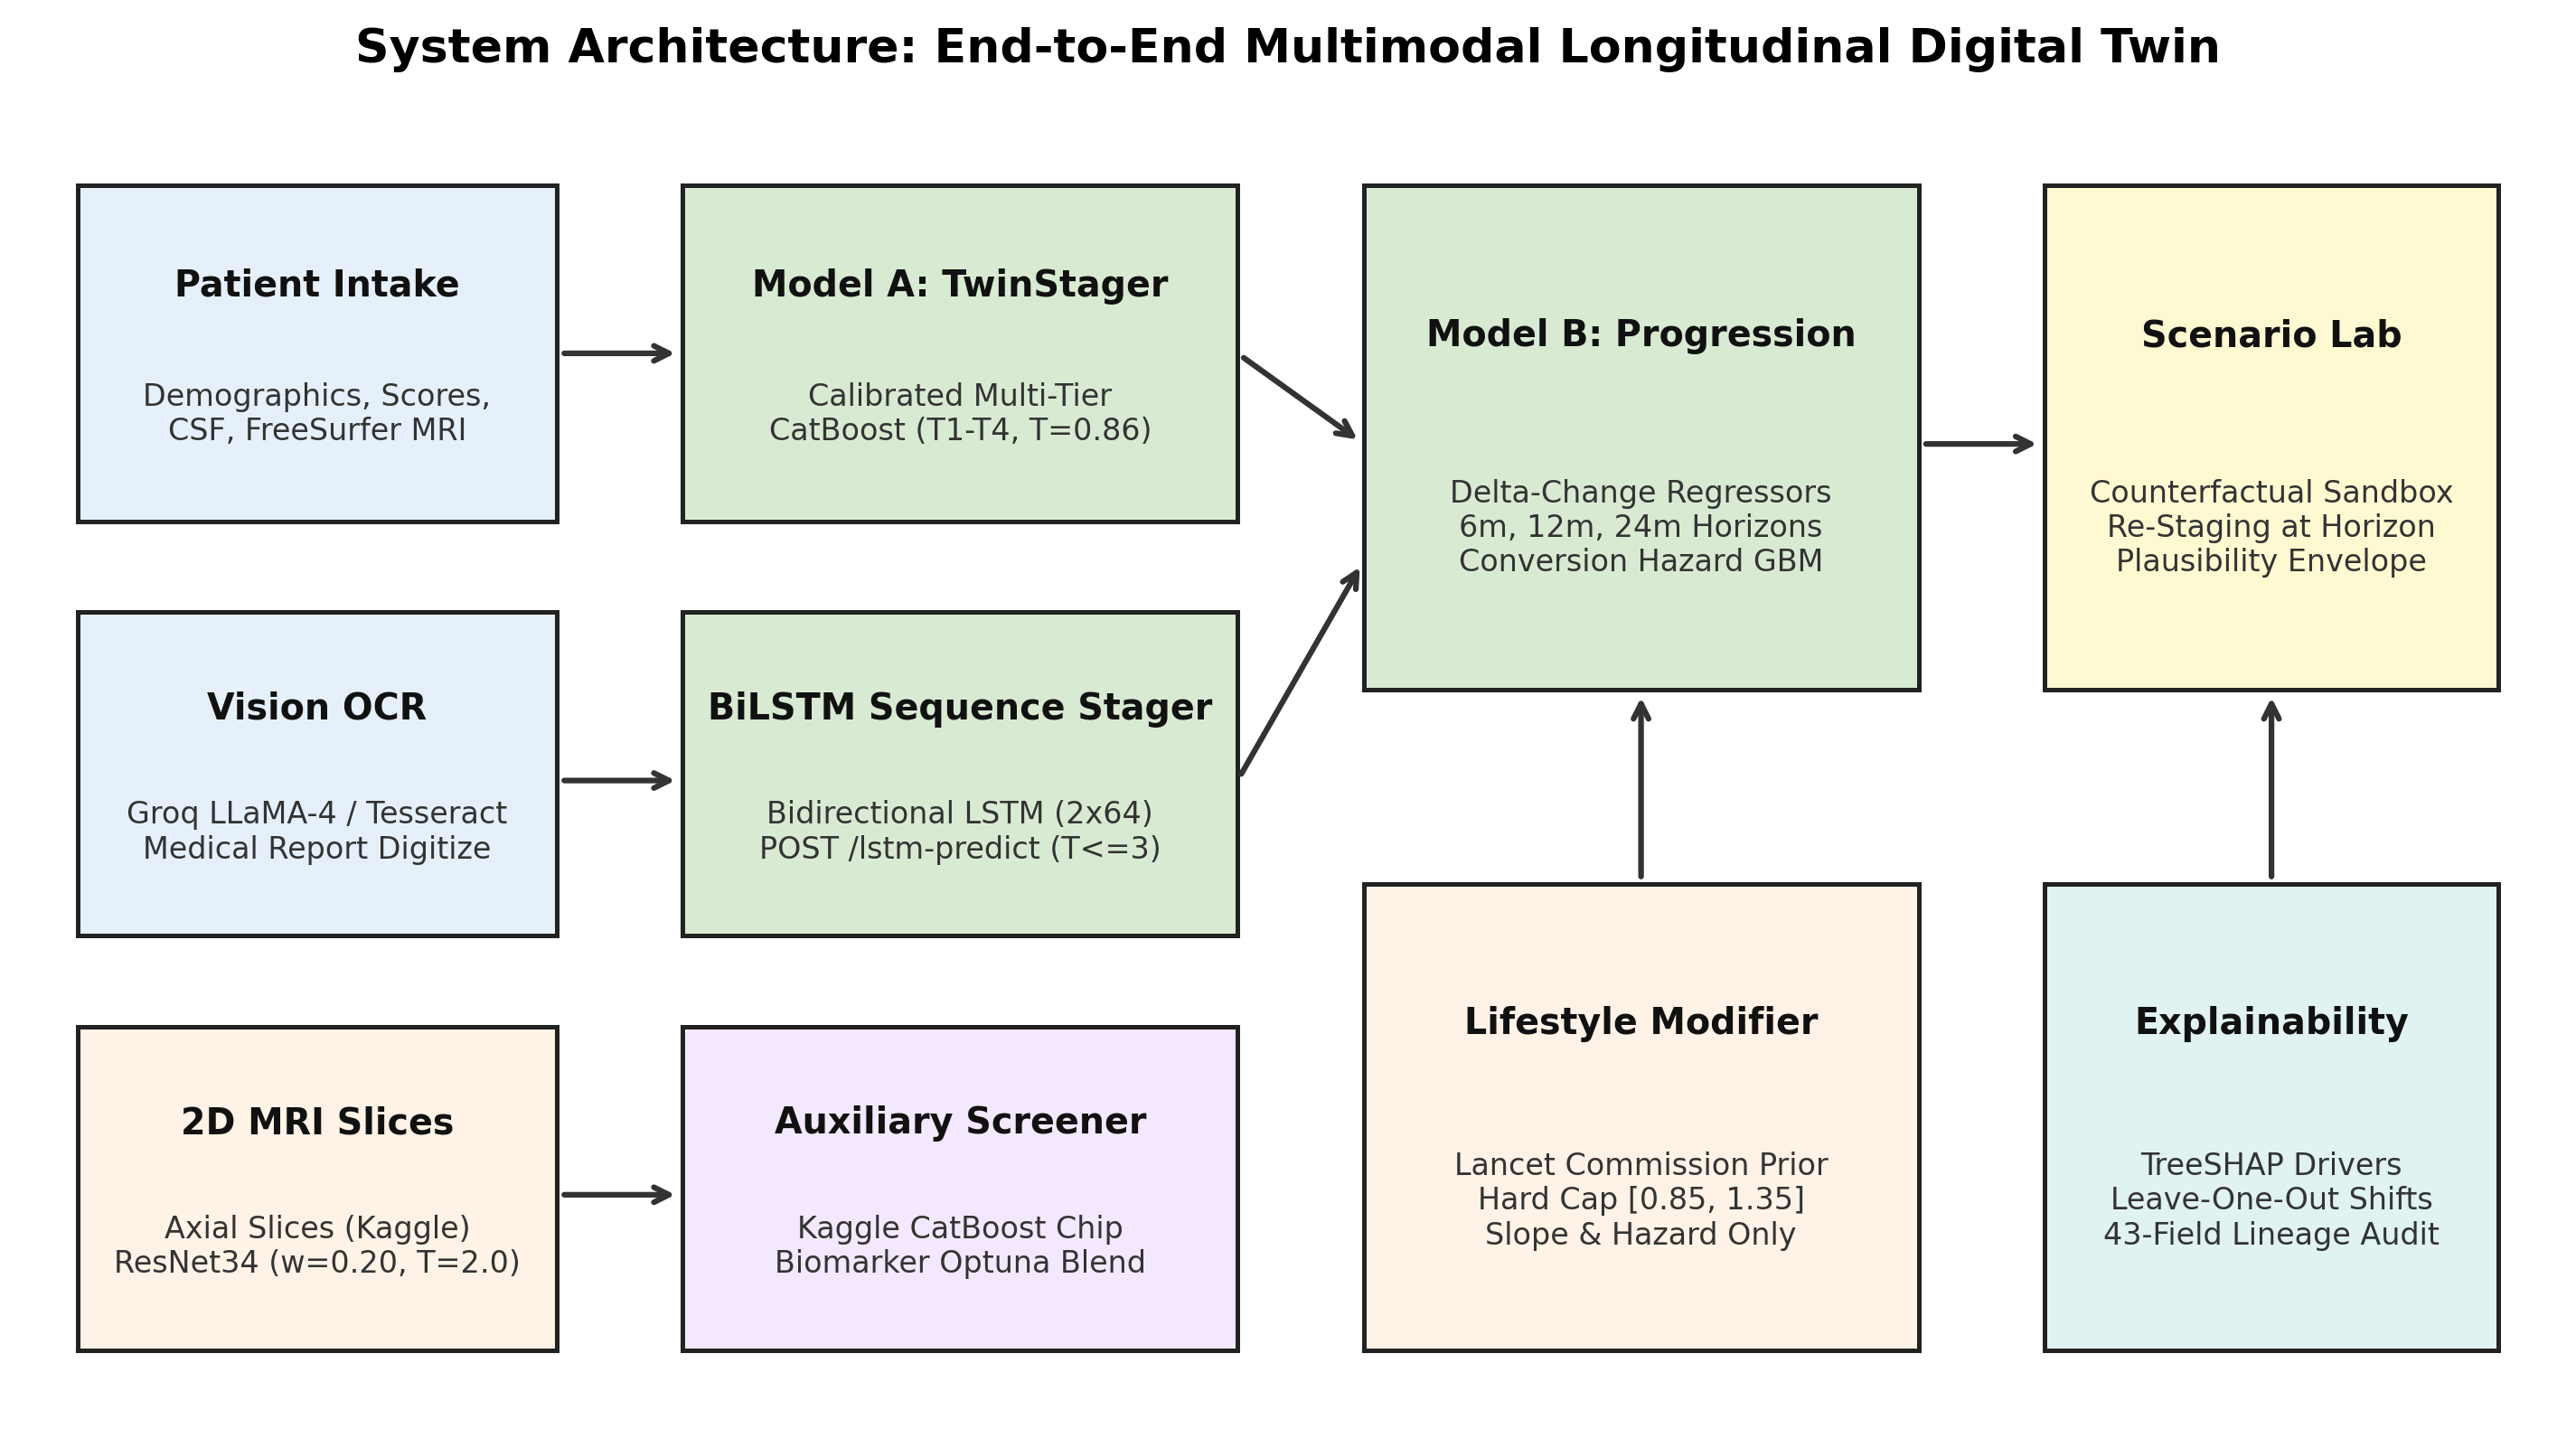
\includegraphics[width=0.95\linewidth]{figures/System_architecture.png}
    \caption{End-to-end system architecture: Multimodal patient intake routes clinical, cognitive, fluid, and imaging data through the calibrated TwinStager (Model A), the multi-horizon progression engine (Model B), and the Counterfactual Scenario Lab, bounded by empirical plausibility guards and TreeSHAP explainability.}
    \label{fig:architecture}
\end{figure}

The pipeline executes through five integrated operational stages:
\begin{enumerate}
    \item \textbf{Intake and Current Stage Detection (Model A)}: Heterogeneous patient observations across demographics, bedside cognitive scores, cerebrospinal fluid (CSF) assays, and structural neuroimaging are ingested without statistical imputation. The calibrated multi-tier TwinStager dynamically identifies the highest clinically valid feature tier and computes calibrated posterior probabilities across Cognitively Normal (CN), Mild Cognitive Impairment (MCI), and Alzheimer's Disease (AD).
    \item \textbf{Longitudinal Progression Tracking (Model B)}: Anchor visit cognitive scores and predicted staging probabilities feed into target-specific delta-change regressors that forecast prospective decline across 6-, 12-, and 24-month horizons for three core cognitive endpoints: the Mini-Mental State Examination (MMSE), the Clinical Dementia Rating Global score (CDGLOBAL), and the Alzheimer's Disease Assessment Scale--Cognitive Subscale (ADAS11-Cog).
    \item \textbf{Conversion Risk Estimation}: For baseline non-demented anchor visits (CN and MCI), binary hazard classifiers estimate the probability of progression to AD across 6, 12, and 24 months. Projected test scores are subsequently re-routed through Model~A to estimate complete future stage probability distributions at each horizon.
    \item \textbf{Sequence-Based Staging (Bidirectional LSTM)}: When a patient presents with multiple historical consultations, a Bidirectional Long Short-Term Memory (BiLSTM) network processes chronological sliding windows ($T \le 3$) to capture temporal momentum and predict syndromic transitions at the subsequent visit.
    \item \textbf{Counterfactual Simulation and Governance}: The Counterfactual Scenario Lab receives projected trajectories, allowing clinicians to perturb cognitive decline velocity or simulate literature-grounded lifestyle interventions. Every projection is audited against an empirical 5th--95th percentile training envelope, physiological boundary guards, TreeSHAP feature attributions, leave-one-modality-out sensitivity shifts, and an explicit 43-field intake lineage matrix.
\end{enumerate}

\subsection{Data, Cohort, and Leakage Controls}
The primary longitudinal dataset was constructed from the Alzheimer's Disease Neuroimaging Initiative (ADNI) repository~\cite{petersen2010adni}, consolidating participants across ADNI-1, ADNI-GO, ADNI-2, and ADNI-3. A master dataset comprising \TotalRows{} clinical visits across \TotalSubjects{} unique participants was compiled by integrating five primary diagnostic modalities: clinical diagnosis consensus records, bedside neuropsychological examination batteries, cerebrospinal fluid molecular assays, ComBat-harmonized FreeSurfer volumetric MRI, and APOE targeted genotyping (Table~\ref{tab:cohort_splits} and Table~\ref{tab:data_sources}).

\begin{table}[t]
\centering
\caption{Cohort summary and subject-level stratified data partition across the Alzheimer's Disease Neuroimaging Initiative (ADNI) unified longitudinal cohort ($N=3,034$ subjects, 22,168 clinical visits).}
\label{tab:cohort_splits}
\small
\begin{tabular}{lrrrrr}
\toprule
\textbf{Split Partition} & \textbf{Subjects} & \textbf{Split Share} & \textbf{Visits} & \textbf{Converters} & \textbf{Converter Share} \\
\midrule
Training Set             & 2,123             & 70.0\%               & 15,488          & 372                 & 17.5\% \\
Validation Set           & 455               & 15.0\%               & 3,486           & 80                  & 17.6\% \\
Held-Out Test Set        & 456               & 15.0\%               & 3,194           & 80                  & 17.5\% \\
\midrule
\textbf{Total Cohort}    & \textbf{3,034}    & \textbf{100.0\%}     & \textbf{22,168} & \textbf{532}        & \textbf{17.5\%} \\
\bottomrule
\end{tabular}
\end{table}

\begin{table}[t]
\centering
\caption{Data inventory, file sizes, longitudinal coverage, and merge decisions across the multimodal repository.}
\label{tab:data_sources}
\small
\begin{adjustbox}{max width=\linewidth}
\begin{tabular}{lp{2.6cm}rrlp{5.0cm}}
\toprule
\textbf{Dataset File} & \textbf{Modality / Family} & \textbf{Size} & \textbf{Visits} & \textbf{Coverage} & \textbf{Merge Decision \& Role} \\
\midrule
\texttt{shortened\_result-val.csv} & Longitudinal DX Ground Truth & 1.02 MB & 22,168 & 100.0\% & Canonical baseline diagnosis backbone (1=CN, 2=MCI, 3=AD). \\
\texttt{ADNIMERGE\_13Aug2025.csv} & Demographics, CSF, PET & 12.65 MB & 16,421 & 77.6\% & Exact VISCODE join + nearest $\pm 2$ months fallback; CSF biomarkers. \\
\texttt{ADSP\_PHC\_T1\_FS\_15Aug2025.csv} & ComBat FreeSurfer MRI & 39.17 MB & 10,260 & 76.3\% & Backward-only temporal merge ($\le 180$ days prior); no future scan leakage. \\
\texttt{All\_Subjects\_APOERES\_fixed\_simple.csv} & APOE Genotyping & 0.22 MB & 3,006 & 85.3\% & Curated APOE strings parsed to numeric $\varepsilon4$ allele count ($0, 1, 2$). \\
\texttt{All\_Subjects\_My\_Table\_30Dec2025.csv} & Neuropsychological Tests & 3.36 MB & 24,759 & 100.0\% & Standardized scores: CDR-SB, MoCA, and FAQ activities. \\
\texttt{All\_Subjects\_Study\_Entry\_30Dec2025.csv} & Study Metadata & 0.22 MB & 4,934 & 100.0\% & Entry baseline age and anchor date for visit timeline reconstruction. \\
\texttt{All\_Subjects\_ADAS\_30Dec2025.csv} & ADAS-Cog Audit File & 1.72 MB & 12,919 & 97.0\% & Audit verification: proves identity $\text{TOTSCORE} \equiv \text{ADAS11 prorated}$ ($r=0.9991$). \\
\texttt{alzheimers\_disease\_data.csv} & Lifestyle Screening (Kaggle) & 0.61 MB & 2,149 & External & Independent cohort; trains separate auxiliary screening chip (unblended). \\
Kaggle 2D MRI Slice Dataset & Axial Neuroimaging Slices & 44,000 imgs & N/A & External & Trains 2D ResNet34; fused at weight $w=0.20$ with temperature $T=2.0$. \\
\bottomrule
\end{tabular}
\end{adjustbox}
\end{table}


To guarantee statistical validity and prevent observational bias, four architectural anti-leakage safeguards were enforced (Fig.~\ref{fig:data_pipeline}):
\begin{enumerate}
    \item \textbf{Subject-Level Stratified Partitioning}: Rather than partitioning records at the visit level, which allows longitudinal visits from the same subject to appear in both training and evaluation partitions, data splitting was performed strictly at the subject level. Partitioning utilized a stratified group split conditioned on participant baseline diagnosis and longitudinal conversion status \texttt{(baseline\_diagnosis, ever\_converted)}. As summarized in Table~\ref{tab:cohort_splits}, \TrainSubjects{} subjects (\TrainPct{}) were allocated to model training, \ValSubjects{} subjects (\ValPct{}) to hyperparameter validation, and \TestSubjects{} subjects (\TestPct{}) to an independent held-out evaluation test set. Converter proportions were exactly matched across partitions (17.5\%), and programmatic assertions verified zero subject overlap between splits.
    \item \textbf{Strict Backward-Only Neuroimaging Temporal Joins}: In routine neurology, neuroimaging is rarely obtained on the exact date of clinical examination. To align imaging with cognitive evaluations without leaking future anatomical deterioration, each cognitive visit was linked exclusively to the most recent volumetric MRI scan acquired on or prior to the visit date. Forward-looking scans (acquired after the examination date) were strictly excluded. Scans acquired more than 180 days prior were treated as unobserved missing entries, preventing temporally decoupled brain morphometry from biasing current staging.
    \item \textbf{Visit Timeline Reconstruction}: Exact clinical examination dates were extracted from recorded visit timestamps (72.0\%) or calculated from recorded baseline anchor dates and protocol visit intervals (28.0\%). Baseline and screening visits occurring within protocol proximity were collapsed to visit month $0.0$, eliminating duplicate baseline anchor points.
    \item \textbf{Forbidden Feature Blacklisting}: Sixteen features encoding full longitudinal history or diagnostic targets were permanently blacklisted. These include total lifetime visit counts, retrospective longitudinal trajectory classifications, imputation confidence flags, and retrospective clinician diagnosis revision codes. Models trained on such variables exhibit artificially inflated test accuracy by inadvertently reading future patient outcomes.
    \item \textbf{Handling Observational Missingness Without Imputation}: In real-world cohorts, diagnostic missingness is non-random; invasive tests such as lumbar punctures or research-grade MRI are administered selectively based on clinical suspicion. Imputing unobserved values via mean, median, or multivariate imputation (MICE) distorts physiological variance and leaks cross-subject future information. We strictly rejected statistical imputation: missing modalities (84.7\% missingness for CSF, 45.5\% for volumetric MRI) were retained as native missing values and routed through tree-split decision logic.
\end{enumerate}

\begin{figure}[H]
    \centering
    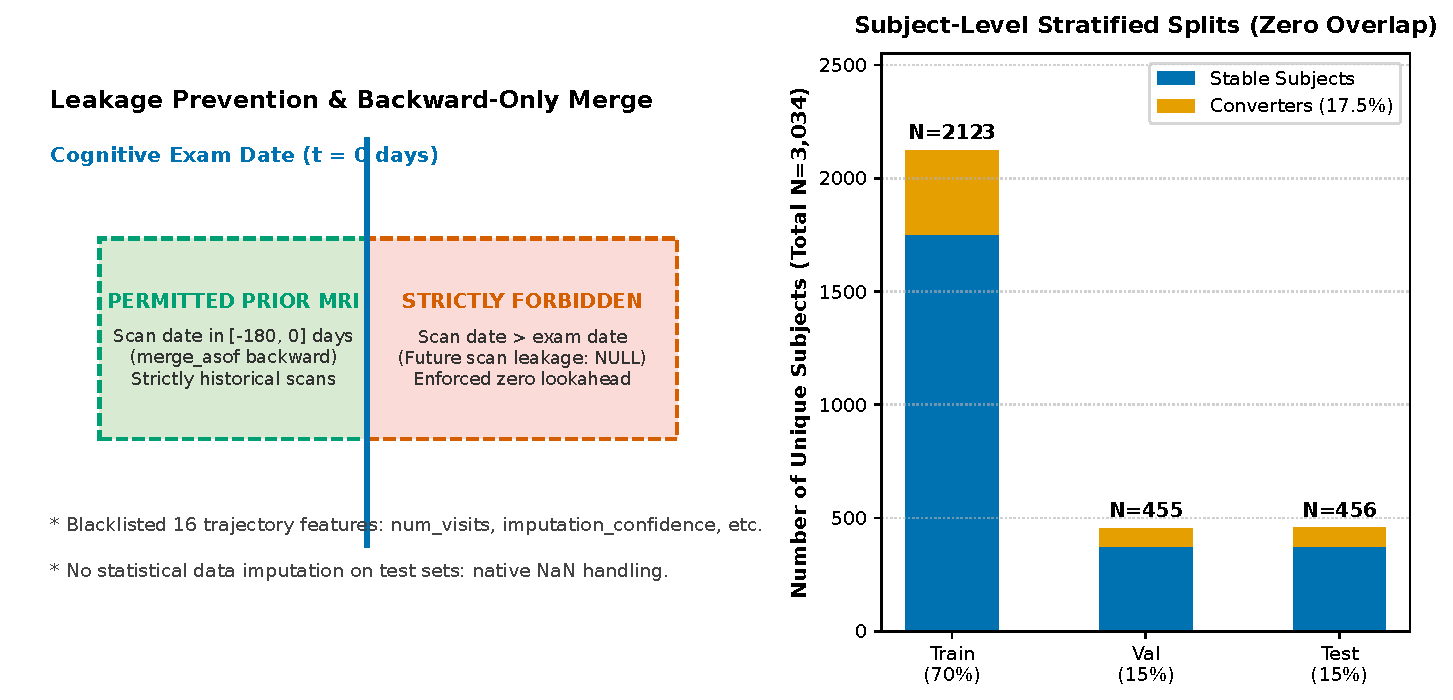
\includegraphics[width=0.95\linewidth]{figures/fig_data_pipeline.pdf}
    \caption{Longitudinal data pipeline and leakage controls: (Left) Strictly backward-only temporal merge enforcing zero future scan attachment ($\le 180$ days); (Right) Subject-level stratified partition preserving converter proportions across splits.}
    \label{fig:data_pipeline}
\end{figure}

\subsection{Step 1, Current Stage Detection: Multi-Tier Stager (Model A)}
Cross-sectional syndromic staging establishes the baseline diagnostic foundation of the digital twin by classifying each clinical consultation into one of three standard clinical categories: Cognitively Normal (CN), Mild Cognitive Impairment (MCI), or Alzheimer's Disease (AD). In real-world clinical practice, diagnostic resources vary substantially—ranging from community clinics equipped only with rapid bedside screening tools to specialized academic memory centers with access to cerebrospinal fluid assays and structural neuroimaging. 

To reflect this clinical reality without resorting to synthetic statistical imputation, Step~1 executes as a modular diagnostic workflow (Fig.~\ref{fig:architecture}):
\begin{enumerate}
    \item \textbf{Data Ingestion and Digitization}: When clinical inputs arrive as unstructured paper records, scanned PDFs, or laboratory printouts, an intake Vision-Language OCR pipeline parses and extracts validated clinical parameters.
    \item \textbf{Dynamic Multi-Tier Tabular Inference}: The primary stager dynamically identifies the highest clinically valid feature tier supported by available patient observations and evaluates calibrated syndromic probabilities.
    \item \textbf{Multimodal Visual Extension}: When a raw 2D structural MRI scan slice is uploaded, a deep convolutional vision head generates image-derived probabilities that are blended with the tabular stager via calibrated late fusion.
    \item \textbf{Auxiliary Molecular Profiling}: When CSF biomarkers and genotyping are present, an auxiliary ensemble provides complementary molecular risk confirmation.
\end{enumerate}

\subsubsection{Dynamic Multi-Tier Feature Routing Architecture}
Rather than requiring complete multimodal profiles or replacing unobserved tests with artificial statistical substitutes, Model~A dynamically evaluates the patient's record at intake and routes inference through the highest valid tier:
\begin{itemize}
    \item \textbf{Tier T1 (Demographics \& Genetics)}: Patient entry age, biological sex, completed education years, and APOE $\varepsilon4$ risk allele count ($0, 1, 2$).
    \item \textbf{Tier T1b (Rapid Bedside Screener)}: Tier T1 augmented with the Mini-Mental State Examination (\texttt{MMSE}), representing routine primary care cognitive screening.
    \item \textbf{Tier T2a (Functional Staging)}: Tier T1b augmented with the Clinical Dementia Rating Global score (\texttt{CDGLOBAL}) and Sum of Boxes (\texttt{CDRSB}), capturing functional independence and daily living impairment.
    \item \textbf{Tier T2b (Core Neuropsychological Battery)}: Tier T2a augmented with detailed neuropsychological test batteries: ADAS11-Cog total score (\texttt{TOTSCORE}), the Functional Activities Questionnaire (\texttt{FAQTOTAL}), and the Montreal Cognitive Assessment (\texttt{MOCA}), capturing fine-grained memory, praxis, and executive function.
    \item \textbf{Tier T3 (+CSF Biomarkers)}: Tier T2b augmented with cerebrospinal fluid molecular assays: amyloid-beta ($\text{A}\beta_{42}$), total tau (t-tau), hyperphosphorylated tau ($\text{p-tau}_{181}$), and lower/upper assay censorship flags.
    \item \textbf{Tier T4 (+FreeSurfer Volumetric MRI)}: Tier T3 augmented with ComBat-harmonized FreeSurfer morphometry, including normalized bilateral hippocampal volume, hippocampal asymmetry, ventricular volume, total brain parenchymal volume, and regional cortical thicknesses.
\end{itemize}

\subsubsection{Core Stager Architecture and Temperature Calibration}
The primary stager is built using a CatBoostClassifier~\cite{prokhorenkova2018catboost}. CatBoost was selected over alternative architectures (e.g., Random Forests, Multi-Layer Perceptrons) because of its native handling of missing numerical values via optimal threshold routing during tree construction, robust handling of heterogeneous tabular distributions, resistance to overfitting via symmetric oblivious decision trees, and millisecond-scale deterministic inference. 

The stager was trained with 600 iterations, a maximum tree depth of 6, a learning rate of 0.05, multiclass cross-entropy loss, and balanced class weights ($1.0$ for CN, $1.5$ for MCI, and $2.0$ for AD) to account for lower relative prevalence of dementia in community cohorts. Early stopping was monitored on the validation partition with a 50-round patience window. To prevent subjects with extensive longitudinal follow-up from dominating the loss objective, sample weights inversely proportional to subject visit counts ($w_i = 1 / N_{\text{visits}}$) were applied during training.

Because raw tree ensemble margin logits frequently exhibit uncalibrated overconfidence, we performed post-hoc calibration via Temperature Scaling—the multi-class generalization of Platt scaling. A scalar temperature parameter $T > 0$ was fitted on the validation partition by minimizing multiclass negative log-likelihood:
\begin{equation}
    P(y = k \mid \mathbf{x}) = \frac{\exp(z_k / T)}{\sum_{j=1}^{K} \exp(z_j / T)}
\end{equation}
where $z_k$ represents the uncalibrated raw margin logit for class $k \in \{\text{CN}, \text{MCI}, \text{AD}\}$. Bounded scalar optimization yielded an optimal temperature of $T = 0.8554$, reducing the overall Expected Calibration Error (ECE) to $\StagerECEFinal{}$. In the main Results (Table~\ref{tab:stager_results}), empirical multi-tier evaluations demonstrate that diagnostic performance scales steadily from Tier T1 (Macro-F1 = \StagerTOneFOne{}) to Tier T4 (Macro-F1 = \StagerTFourFOne{}).

\subsubsection{Unstructured Intake: Vision-Language OCR Pipeline}
In real-world memory clinics, diagnostic assessments and laboratory panels frequently arrive as unstructured paper documents, scanned clinical reports, or PDF printouts. To eliminate error-prone manual transcription and bridge the gap between unstructured records and tabular inference, the intake engine incorporates a Vision-Language Optical Character Recognition (OCR) pipeline combining Vision-LLaMA Maverick with a local Tesseract fallback. 

The OCR engine processes scanned reports to extract 12 structured clinical parameters (patient age, biological sex, MMSE score, CSF $\text{A}\beta_{42}$, total tau, phosphorylated tau, and APOE genotype) into standardized clinical JSON. Extracted entities are presented in an interactive clinical verification interface, enforcing a mandatory \textit{human-in-the-loop} validation step before parameters are ingested into Model~A or Model~B.

\subsubsection{2D Structural MRI Classifier and Calibrated Late Fusion}
While Tier~T4 processes numerical FreeSurfer volumetric summaries, clinical encounters often possess only raw 2D neuroimaging scans (e.g., JPEG or PNG slices). To incorporate visual morphological features without requiring full 3D volumetric preprocessing pipelines, the architecture incorporates a deep convolutional vision head based on ResNet-34~\cite{he2016resnet}. The network was fine-tuned via transfer learning on approximately 44,000 augmented 2D axial T1-weighted MRI slices across four nominal stages: Non-Demented, Very Mild Impairment, Mild Impairment, and Moderate Impairment.

To harmonize the vision model with the 3-class syndromic taxonomy of Model~A, visual predictions are mapped as: $\text{Non-Demented} \to \text{CN}$, $\text{Very Mild} \to \text{MCI}$, and $\{\text{Mild}, \text{Moderate}\} \to \text{AD}$. To prevent overconfident deep neural probability spikes from overriding clinical test batteries, visual logits are calibrated with temperature scaling ($T = 2.0$), yielding smoothed probabilities $\mathbf{P}_{\text{mri\_mapped}}$. When an MRI scan is uploaded, the final syndromic posterior distribution $\mathbf{P}_{\text{final}}$ is synthesized via linear late fusion:
\begin{equation}
    P_{\text{final}}(y = k \mid \mathbf{x}) = (1 - w_{\text{mri}}) \cdot P_{\text{adni}}(y = k \mid \mathbf{x}) + w_{\text{mri}} \cdot P_{\text{mri\_mapped}}(y = k \mid \mathbf{x})
\end{equation}
where the image weight is conservatively constrained to $w_{\text{mri}} = 0.20$.

\textbf{Safeguard Rationale}: Public 2D slice datasets often exhibit inflated internal test accuracy ($99.7\%$) arising from slice-level patient overlap across partitions. Heavily down-weighting the visual channel ($w_{\text{mri}} = 0.20$) ensures that rigorous, leak-free tabular clinical scores dominate the diagnostic decision, while visual features provide an auxiliary structural prior accompanied by a persistent UI transparency disclaimer.

\subsubsection{Auxiliary Biomarker Ensemble}
When detailed CSF molecular assays and targeted APOE genotyping are available, an auxiliary Biomarker Ensemble provides molecular risk stratification. Built as an Optuna-optimized blend of Extreme Gradient Boosting (XGBoost), Random Forest, and a Multi-Layer Perceptron (MLP), this chip evaluates non-linear molecular interactions ($\text{A}\beta_{42}/\text{p-tau}_{181}$ ratios and APOE $\varepsilon4$ allele dose) as a secondary diagnostic confirmation tool without altering core tabular clinical staging.

\subsection{Step 2, Progression Tracking: Multi-Horizon Delta Regression (Model B)}
Forecasting future cognitive decline is challenging because predicting absolute test scores ($\hat{y}_{t+h}$) directly often leads to compounding baseline drift. To anchor predictions to the patient's current disease state, Model~B is formulated as a delta-change regression model:
\begin{equation}
    \Delta y_{t, h} = y_{t+h} - y_t, \quad h \in \{6, 12, 24\text{ months}\}
\end{equation}
The future predicted score is reconstructed by adding the estimated change to the baseline anchor value: $\hat{y}_{t+h} = y_t + \widehat{\Delta y}_{t, h}$.

We selected three primary cognitive and functional endpoints:
\begin{enumerate}
    \item \textbf{MMSE} ($0$--$30$ scale): The primary clinical benchmark for global cognitive tracking;
    \item \textbf{CDGLOBAL} ($0$--$3$ scale): The standard ordinal measure of functional independence;
    \item \textbf{ADAS11-Cog} ($0$--$70$ scale): The primary cognitive endpoint in Alzheimer's disease pharmacological clinical trials.
\end{enumerate}
Progression horizons of 6, 12, and 24 months were selected to align with standard clinical follow-up schedules and therapeutic trial endpoints. For each endpoint and horizon, an independent CatBoostRegressor was trained on all valid anchor visits possessing an observed evaluation at horizon $h$. 

\subsubsection{Feature Representation and Lineage Routing}
In the clinical deployment demo, intake captures a comprehensive 43-field patient record; however, rather than unrestrictedly passing all 43 intake variables into regression trees, Model~B enforces strict feature lineage (Table~\ref{tab:lineage_summary}):
\begin{enumerate}
    \item \textbf{Direct Model Inputs (Only 10 Features Feed CatBoost)}: These represent the only variables from which the CatBoost regression models calculate future cognitive decline curves:
    \begin{itemize}
        \item \textit{Demographics \& Genetics (4 features)}: Patient entry age, biological sex, completed education years, and APOE $\varepsilon4$ risk allele count ($0, 1, 2$).
        \item \textit{Cognitive \& Functional Assessments (6 features)}: Mini-Mental State Examination (\texttt{MMSE}), Clinical Dementia Rating Global score (\texttt{CDGLOBAL}), CDR Sum of Boxes (\texttt{CDRSB}), ADAS11-Cog prorated total score (\texttt{TOTSCORE}), Functional Activities Questionnaire (\texttt{FAQTOTAL}), and Montreal Cognitive Assessment (\texttt{MOCA}).
        \item \textit{Optional Volumetric Neuroimaging}: When structural neuroimaging is available, the model can optionally evaluate ComBat-harmonized FreeSurfer morphometry (normalized bilateral hippocampal volume, hippocampal asymmetry, ventricular volume, total brain parenchymal volume, and regional cortical thicknesses).
    \end{itemize}
    \item \textbf{External Velocity Multipliers (10 Lifestyle \& Medical History Factors)}: An additional ten modifiable lifestyle and vascular risk factors—current smoking, physical inactivity, alcohol consumption, diet quality, sleep disturbance, midlife hypertension, type~2 diabetes, depression, traumatic brain injury, and cardiovascular disease—do \textit{not} enter the machine learning model directly. Because ADNI did not record longitudinal lifestyle logs, treating them as direct tree features would risk synthetic bias. Instead, they act as an external velocity multiplier via the Lancet Commission relative-risk prior ($M_{\text{lifestyle}} \in [\LifestyleHardCapLo{}, \LifestyleHardCapHi{}]$), scaling the predicted decline slope ($\Delta y_{\text{adj}} = \Delta y_{t,h} \cdot M_{\text{lifestyle}}$) to show steeper prospective decline when multiple comorbidities co-occur and modulating 24-month conversion hazard.
    \item \textbf{Quarantined and Chart-Only Fields (23 Variables)}: Physical vitals (height, weight, BMI) are stored for clinical tracking only (empirical vitals ablation demonstrated $\Delta\text{MAE} = -0.0080$, $p > 0.05$); nine subjective symptoms (e.g., memory complaints, confusion, disorientation) feed an auxiliary screening questionnaire chip; and administrative metadata (e.g., patient name, doctor, baseline calendar date) remain strictly quarantined from all prognostic algorithms.
\end{enumerate}

To assess performance, Model~B was evaluated against two established prognostic baselines:
\begin{itemize}
    \item \textbf{Naive Persistence Baseline}: Assumes zero future change ($\widehat{\Delta y}_{t, h} = 0$, $\hat{y}_{t+h} = y_t$), representing the hypothesis that patient status remains static;
    \item \textbf{Linear Slope Extrapolation}: Computes the patient's historical annualized rate of change across prior visits ($\ge 2$ visits) and extrapolates linearly across horizon $h$.
\end{itemize}

Prediction intervals (90\% and 95\% confidence bounds) were generated using 1,000 cluster-bootstrap iterations resampled at the subject level. Resampling entire subject clusters with replacement accounts for repeated-measures intra-subject correlation, preventing the artificially narrowed confidence intervals produced by naive sample-level bootstrapping. As reported in Section~\ref{sec:results} (Table~\ref{tab:forecast_mae}), Model~B achieves an MAE of \MMSEMAEXII{} points for 12-month MMSE decline, significantly outperforming persistence (\MMSEPersistXII{}) and slope extrapolation (\MMSESlopeXII{}).

\subsection{Step 3, Conversion Risk Estimation}
A vital clinical task is predicting which non-demented patients will progress to dementia. Conversion risk estimation is restricted strictly to non-demented baseline anchor visits (Cognitively Normal and Mild Cognitive Impairment). Patients already diagnosed with Alzheimer's disease at the anchor visit are ineligible for conversion modeling, as they have already reached the dementia endpoint; for these patients, the progression engine instead evaluates rapid functional decline risk (probability of losing $\ge 3$ MMSE points).

For each horizon $h \in \{6, 12, 24\}$ months, a binary CatBoostClassifier was trained to predict whether an initial CN or MCI anchor will convert to AD within that window. Models were evaluated using two complementary metrics:
\begin{enumerate}
    \item \textbf{Area Under the Receiver Operating Characteristic (AUROC)}: Quantifies threshold-independent discrimination between converters and stable non-converters;
    \item \textbf{Brier Skill Score (BSS)}: Evaluates probabilistic calibration and refinement relative to a baseline reference forecast ($\text{BSS} = 1 - \text{BS} / \text{BS}_{\text{ref}}$). A positive BSS demonstrates that model probabilities outperform historical empirical incidence rates.
\end{enumerate}

To complete the longitudinal trajectory projection, projected cognitive scores ($\hat{y}_{t+h}$) are passed back into the calibrated TwinStager (Model A). This produces re-staged diagnostic posterior probabilities ($P(\text{CN})$, $P(\text{MCI})$, $P(\text{AD})$) at each future horizon, allowing clinicians to inspect expected syndromic transition timelines alongside continuous numerical decline (Section~\ref{sec:results}, Table~\ref{tab:conversion_metrics}, reaching AUROC of \ConvAUCXXIV{} and BSS of \ConvBSSXXIV{} at 24 months).

\subsection{Step 4, Sequence-Based Staging: Bidirectional LSTM}
\label{sec:bilstm_methodology}
A fundamental architectural distinction separates Step~2 (Model B: Longitudinal Progression Tracking) from Step~4 (Sequence-Based Staging: BiLSTM):
\begin{itemize}
    \item \textbf{Step 2 (Model B: Multi-Horizon Continuous Regression)}: Takes a \textit{single static anchor visit} ($t$) comprising tabular demographic features, baseline cognitive batteries, optional fluid/imaging biomarkers, and Model~A's baseline stage probabilities. It outputs \textit{continuous numeric score changes} ($\Delta y_{t,h}$ for MMSE, CDGLOBAL, and ADAS11) across fixed calendar horizons ($h \in \{6, 12, 24\}$ months) to reconstruct future disease severity curves ($\hat{y}_{t+h} = y_t + \widehat{\Delta y}_{t,h}$) with 95\% cluster-bootstrap uncertainty intervals.
    \item \textbf{Step 4 (Sequence Staging: Bidirectional LSTM)}: Takes a \textit{multi-visit chronological trajectory} across a sliding sequence of up to $T \le 3$ consecutive clinical consultations ($\mathbf{X} \in \mathbb{R}^{B \times T \times D}$). Rather than predicting continuous numeric deltas at fixed time intervals, it outputs a \textit{discrete 3-class syndromic stage distribution} ($P(\text{CN})$, $P(\text{MCI})$, $P(\text{AD})$) at the subsequent clinical follow-up visit ($t+1$), capturing whether the cumulative velocity of past cognitive changes heralds a diagnostic syndromic transition.
\end{itemize}

Each consultation in the input sequence tracks $D = 5$ standardized longitudinal features: patient entry age, CDR global score (\texttt{CDGLOBAL}), Mini-Mental State Examination (\texttt{MMSCORE}), ADAS-Cog-11 prorated score (\texttt{TOTSCORE}), and elapsed visit month (\texttt{visit\_month}). Sequences with fewer than three visits are pre-padded along the temporal dimension ($T=3$). Features are normalized using an empirical Min-Max scaler fitted exclusively on the training partition.

\subsubsection{Observation Masking vs. Zero-Imputation Formulation}
A central challenge in sequential clinical modeling is handling missing observations across longitudinal visits. We compared two input formulations:
\begin{enumerate}
    \item \textbf{Zero-Imputed Baseline ($D = 5$ channels)}: Unobserved feature values and pre-padded time steps are set to zero: $\mathbf{x}_t \in \mathbb{R}^5$. However, this conflates true physiological zero scores (e.g., $\text{CDGLOBAL} = 0$, indicating cognitively normal status) with unobserved tests.
    \item \textbf{Binary-Masked Representation ($2D = 10$ channels)}: An explicit binary observation mask vector $\mathbf{m}_t \in \{0, 1\}^5$ is concatenated to the feature vector at each time step ($m_{t, j} = 1$ if feature $j$ was observed at visit $t$, and $0$ if missing or padded): $\tilde{\mathbf{x}}_t = [\mathbf{x}_t \parallel \mathbf{m}_t] \in \mathbb{R}^{10}$. This provides explicit missingness indicators directly to the recurrent input and forget gates.
\end{enumerate}

The network architecture consists of:
\begin{enumerate}
    \item A Bidirectional LSTM layer with 64 forward and 64 backward recurrent units ($128$ concatenated recurrent channels, input dropout $0.2$, recurrent dropout $0.1$) to capture both past deficit accumulation and retrospective rate-of-change;
    \item A Batch Normalization layer stabilizing hidden state activations across variable-length sequence inputs;
    \item A fully-connected Dense layer with 32 rectified linear units (ReLU) and $L_2$ kernel weight regularization ($\lambda = 10^{-4}$);
    \item A Dropout regularization layer ($p = 0.3$);
    \item A 3-unit Softmax classification layer computing posterior probabilities for CN, MCI, and AD at the subsequent clinical visit.
\end{enumerate}
The BiLSTM was trained on ADNI consultation sequences using the Adam optimizer ($\text{learning rate} = 10^{-3}$, batch size 32) and sparse categorical cross-entropy loss with balanced inverse-frequency class weights.

\subsubsection{Empirical Sequential Staging Comparison}
To evaluate the impact of explicit observation masking and determine whether recurrent sequence modeling justifies replacing gradient-boosted decision trees, we conducted a paired benchmark across $N = 1{,}340$ sliding sequence windows from $589$ held-out test subjects (Table~\ref{tab:bilstm_mask_comparison}).

\begin{table}[H]
\centering
\small
\caption{Empirical comparison of sequential staging architectures on the held-out subject-level test cohort ($N = 1{,}340$ sliding windows across 589 subjects).}
\label{tab:bilstm_mask_comparison}
\begin{tabular}{llccc}
\toprule
\textbf{Model Architecture} & \textbf{Input Strategy} & \textbf{Test Accuracy} & \textbf{Macro-F1} & \textbf{Log Loss} \\
\midrule
Zero-Imputed BiLSTM (5 feat) & Zero-imputation ($0.0$) & 83.43\% & 0.8291 & 0.4592 \\
Binary-Masked BiLSTM (10 feat) & Values + Binary Masks ($\mathbf{x}_t \parallel \mathbf{m}_t$) & 84.03\% & 0.8364 & 0.4410 \\
CatBoost (Model A / Stager) & Natural missingness (\texttt{NaN} routing) & \textbf{84.63\%} & \textbf{0.8427} & \textbf{0.3980} \\
\bottomrule
\end{tabular}
\end{table}

This empirical evaluation reveals two critical findings:
\begin{enumerate}
    \item \textbf{Binary Masking Improves Recurrent Sensitivity}: Supplying the explicit binary mask $\mathbf{m}_t$ improves BiLSTM Macro-F1 from $0.8291$ to $0.8364$ ($+0.0073$) and lowers predictive cross-entropy log loss from $0.4592$ to $0.4410$. In particular, Alzheimer's disease recall improves by $+2.17\%$ (from 81.16\% to 83.33\%, with F1 rising from $0.7986$ to $0.8142$), while MCI recall is preserved at 79.00\% (F1: $0.7929 \to 0.7989$) and CN F1 remains stable ($0.8959 \to 0.8963$). Explicit masks prevent the recurrent memory cells from misinterpreting omitted tests as asymptomatic baseline zeros.
    \item \textbf{CatBoost Retains Superior Tabular Discrimination}: Despite the gains achieved by binary masking, CatBoost with native missingness routing still outperforms both BiLSTM variants, achieving the highest overall test accuracy (84.63\%), superior Macro-F1 (0.8427), highest AD recall (84.42\%, F1: 0.8219), highest MCI recall (79.55\%, F1: 0.8060), and significantly sharper probability calibration (log loss of $0.3980$ vs. $0.4410$).
\end{enumerate}

\subsubsection{Architectural Adoption Rationale}
CatBoost was selected as the primary operational engine for Model~A (staging) and Model~B (progression) for four reasons:
\begin{itemize}
    \item \textbf{Thresholded Decision Boundaries}: Clinical staging metrics (e.g., $\text{CDGLOBAL} \ge 0.5$, $\text{MMSE} \le 24$) follow step-function diagnostic rules that decision trees partition along orthogonal split axes without requiring continuous embedding mappings.
    \item \textbf{Native Missingness Logic}: Tree ensembles route missing values through dedicated split branches during tree construction, avoiding the weight-mask co-adaptation required by continuous neural layers.
    \item \textbf{Sequence Length Constraints}: In routine outpatient neurology, patients typically present with short histories ($T \le 3$ visits spaced 6 to 12 months apart). Over such short horizons, non-linear feature interactions across the most recent visit provide stronger prognostic leverage than recurrent hidden state transitions.
    \item \textbf{Operational Efficiency}: CatBoost delivers deterministic, sub-5ms CPU inference and lower uncertainty without GPU dependencies. The BiLSTM is therefore retained as a secondary multi-visit validation module rather than replacing the primary tabular stager.
\end{itemize}

\subsection{Recurrent Regression Experiment (Masked GRU)}
To investigate whether deep recurrent architectures could replace gradient boosted decision trees for continuous multi-horizon numerical regression across irregularly spaced visits, we conducted an empirical experiment with a two-layer Gated Recurrent Unit incorporating missingness indicator masks ($m_t \in \{0, 1\}$)~\cite{che2018grud}. The model was designed to handle observational visit sparsity by concatenating observation masks and time intervals into hidden state transitions.

A pre-defined architectural adoption criterion required the deep recurrent model to achieve a Macro-F1 improvement $\ge 0.03$ and lower MMSE MAE at 12 months on the held-out test partition before replacing CatBoost. While the masked GRU achieved an MMSE 12-month test MAE of \GRUMaskedMAE{} (significantly outperforming an unmasked recurrent GRU baseline of \GRUUnmaskedMAE{}, paired $\Delta = \GRUPairedDelta{}$, $p < 0.05$), CatBoost achieved a superior MAE of \GBMProgressionMAE{} points while delivering deterministic, sub-5ms CPU inference without requiring GPU infrastructure. Consequently, CatBoost was retained for the operational progression engine.

\subsection{Counterfactual Scenario Lab, Plausibility Envelope, and Lifestyle Modifier}
The Counterfactual Scenario Lab provides clinicians with an interactive simulation sandbox to test hypothetical risk modifications without altering the patient's official electronic record. Clinicians can adjust baseline cognitive scores or modulate expected decline velocity using an acceleration multiplier ($\alpha \in [0.5, 1.5]$).

To protect against implausible mathematical extrapolations, all scenario forecasts are bounded by three layers of clinical safeguards:
\begin{enumerate}
    \item \textbf{Empirical Training Envelope}: Derived from the 5th and 95th percentiles of the ADNI training cohort across anchor variables (Table~\ref{tab:archetype_plausibility}): age $[60.7, 84.7]$, MMSE $[20.0, 30.0]$, CDGLOBAL $[0.0, 1.0]$, and ADAS11 $[2.3, 26.3]$. When patient inputs fall outside these empirical boundaries, automated scope alerts are generated and prediction interval widths are expanded by $1.5\times$ to reflect elevated uncertainty.
    \item \textbf{Physiological Score Caps}: Predictions are bounded strictly to valid clinical assessment scales ($\text{MMSE} \in [0, 30]$, $\text{CDGLOBAL} \in [0, 3]$, $\text{ADAS11} \in [0, 70]$).
    \item \textbf{Biological Monotonicity Bounds}: Untreated neurodegenerative decline does not experience spontaneous physiological recovery. For patients staged as MCI or AD, positive MMSE changes are bounded to $\Delta \le +1.0$ point/year; for patients with advanced dementia ($\text{MMSE} \le 17$), positive score drift is restricted to zero.
\end{enumerate}

\begin{table}[t]
\centering
\caption{Clinical archetype benchmark: validation against empirical 5th--95th percentile training envelope and automated scope guards.}
\label{tab:archetype_plausibility}
\small
\begin{adjustbox}{max width=\linewidth}
\begin{tabular}{lp{3.2cm}rrrrp{3.5cm}}
\toprule
\textbf{Archetype} & \textbf{Baseline Scores} & \textbf{P(CN)} & \textbf{P(MCI)} & \textbf{P(AD)} & \textbf{12m MMSE [Bounds]} & \textbf{Reliability \& Scope Alerts} \\
\midrule
Cognitively Normal (CN) & Age 72, MMSE 29, CDR 0, ADAS 5, FAQ 0   & \textbf{0.933} & 0.053 & 0.014 & 28.5 [26.1, 30.0] & \texttt{ok}; no scope alerts. \\
Mild Cognitive Imp (MCI)& Age 72, MMSE 27, CDR 0.5, ADAS 10, FAQ 3 & 0.025 & \textbf{0.933} & 0.041 & 25.8 [23.4, 28.3] & \texttt{ok}; no scope alerts. \\
Mild AD                 & Age 72, MMSE 20, CDR 1.0, ADAS 25, FAQ 15& 0.011 & 0.030 & \textbf{0.959} & 13.9 [$\le \text{curr}+1$] & \texttt{ok}; valid advanced decline. \\
Moderate AD             & Age 72, MMSE 16, CDR 1.0, ADAS 35, FAQ 18& 0.029 & 0.133 & \textbf{0.838} & 12.3 [$\le \text{curr}+1$] & \texttt{low}; alerts: MMSE 16 outside [20, 30]; ADAS 35 outside [2.3, 26.3]. \\
\bottomrule
\end{tabular}
\end{adjustbox}
\end{table}


Because ADNI does not collect comprehensive longitudinal lifestyle logs, modifiable risk factors cannot be learned directly from cohort data without introducing synthetic bias. Instead, modifiable risks are incorporated via an external, literature-grounded prior derived from the Lancet Commission on Dementia Prevention, Intervention, and Care~\cite{livingston2020lancet,livingston2024lancet}. Ten modifiable risk factors are parameterized with pooled relative risks (RR) from international meta-analyses (Table~\ref{tab:lifestyle_factors}): current smoking ($\text{RR}=1.59$), physical inactivity ($\text{RR}=1.39$), excessive alcohol ($\text{RR}=1.19$), poor diet ($\text{RR}=1.20$), sleep disturbance ($\text{RR}=1.25$), midlife hypertension ($\text{RR}=1.61$), type 2 diabetes ($\text{RR}=1.52$), depression ($\text{RR}=1.91$), traumatic brain injury ($\text{RR}=1.78$), and cardiovascular disease ($\text{RR}=1.28$).

To prevent multiplicative compounding from inflating risk estimates when multiple comorbidities co-occur, relative risks are attenuated using square-root shrinkage ($\text{RR}_{\text{adj}} = \text{RR}^{\LifestyleShrinkage{}}$) and bounded by a conservative hard cap:
\begin{equation}
    M_{\text{lifestyle}} = \text{clip}\left(\prod_{i} \text{RR}_{i}^{\LifestyleShrinkage{}}, \, \LifestyleHardCapLo{}, \, \LifestyleHardCapHi{}\right)
\end{equation}
\textbf{Invariance Safeguard:} The lifestyle multiplier modulates prospective cognitive decline rates and conversion hazard probabilities only; it is mathematically barred from altering baseline syndromic staging probabilities.

\subsection{Explainability and Lineage Governance}
To ensure clinical transparency and support medical decision-making, the framework implements three interpretability mechanisms:
\begin{enumerate}
    \item \textbf{TreeSHAP Feature Attributions}: Exact Shapley additive explanations~\cite{lundberg2017shap} compute feature-level marginal contributions to CatBoost log-odds margins. For each prediction, attributions decompose the model's decision into positive and negative directional forces pushing toward CN, MCI, or AD.
    \item \textbf{Leave-One-Modality-Out Sensitivity Analysis}: For multimodal intakes, advanced diagnostic modalities (CSF biomarkers, volumetric MRI, detailed neuropsychological batteries) are sequentially suppressed to evaluate counterfactual stage probability shifts $\Delta P(\text{Stage})$. This reveals to clinicians whether invasive lumbar punctures or expensive MRI scans alter the diagnostic outcome relative to non-invasive cognitive tests alone.
    \item \textbf{43-Field Intake Lineage Matrix}: Every clinical variable collected at intake is mapped to an explicit system lineage tag (\texttt{used\_in\_stage}, \texttt{used\_in\_forecast}, \texttt{used\_in\_lifestyle}, \texttt{used\_in\_symptom}, \texttt{used\_in\_mri\_fusion}, \texttt{recorded\_only}) (Table~\ref{tab:lineage_summary}). This audit trail ensures that every variable's role is traceable, preventing unauthorized feature leakage between models.
\end{enumerate}

\subsection{Integration of Component Models and Contribution}
The system architecture coordinates the flow of variables and predictions across models:
\begin{itemize}
    \item Intake observations are routed to Model~A, which generates calibrated baseline stage probabilities;
    \item Baseline cognitive scores and Model~A stage probabilities pass to Model~B, which projects delta trajectories and conversion hazards;
    \item Multi-visit consultation histories are evaluated concurrently by the BiLSTM to provide sequential trajectory validation;
    \item Forecasted trajectories pass to the Counterfactual Scenario Lab, where literature-grounded lifestyle priors modulate decline rates within the empirical plausibility envelope;
    \item Interpretability modules extract TreeSHAP drivers, marginal modality shifts, and lineage audits across the entire flow.
\end{itemize}

The principal contributions of this integrated methodology are:
\begin{enumerate}
    \item A leak-free longitudinal data architecture enforcing subject-level partitioning, backward-only imaging joins ($\le 180$ days), and feature blacklisting without statistical imputation;
    \item A calibrated multi-tier routing stager that adapts dynamically to arbitrary clinical data availability;
    \item Open and transparent paired statistical evaluation demonstrating the lack of incremental utility for invasive CSF biomarkers and volumetric MRI;
    \item An audited counterfactual simulation environment bounded by empirical training percentiles and literature-grounded priors.
\end{enumerate}
